\chapter{วรรณกรรมและทฤษฎีบทที่เกี่ยวข้อง}
\section{การต่อเติมภาพเฉดเทา}

\hspace{1cm} ในการกล่าวถึงขั้นตอนวิธีการต่อเติมภาพ จะเริ่มต้นด้วยการกล่าวทบทวนเกี่ยวกับการต่อเติมภาพเฉดสีเทา (grayscale image) ก่อน ดังนี้

\hspace{1cm} ให้ $\Omega \subset \mathbb{R}^2$ แทนโดเมนภาพ (image domain) $D \subset \mathbb{R}^2$ แทนโดเมนต่อเติม (ดูรูปที่ \ref{image:sample-domain}) และ $V \subset [0,\infty)$ และให้ $ u: \Omega \rightarrow V,\ z: \Omega \rightarrow V$ แทนภาพที่ได้รับการซ่อมแซมและภาพที่ต้องการซ่อมแซม ตามลำดับ

\hspace{1cm} ในที่นี้ $ \mathbf{x} = (x,y) \in \Omega $ แทนพิกัดทางกายภาพ (physical position) ของภาพ และ $ u(\mathbf{x}) \in V $ แทนระดับความเข้มของภาพ (image intensity) ที่ $ \mathbf{x} $ และ $ \Omega $ มีรูปร่างสี่เหลี่ยม 

\hspace{1cm} นอกจากนี้เราสามารถสมมติได้โดยไม่เสียหลักการสำคัญว่า $ \Omega = [1,n]^2 $ และ $ V = [0,1] $ เมื่อ $n>0$ เป็นจำนวนเต็มบวก ทั้งนี้ เราจะเรียกภาพ $u,z$ ที่นิยามข้างต้นว่าภาพเฉดสีเทา
\begin{figure}[H]
	\centering
	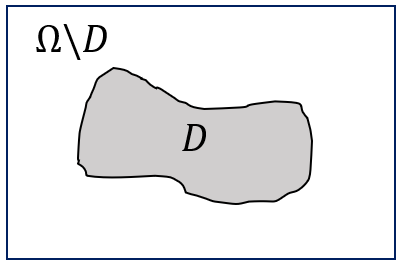
\includegraphics[width=0.375\linewidth]{image/sample-domain.png}
	\caption{$D$ แทนโดเมนต่อเติม}
	\label{image:sample-domain}
\end{figure}

\subsection{ตัวแบบการต่อเติมภาพเฉดสีเทาที่ใช้การแปรผันรวม}\label{inpaint-model-grayscale}

\hspace{1cm} ในการต่อเติมภาพเฉดสีเทา Chan และ Shen \cite{ref:rof-inpaint-chan-shen} ได้นำเสนอตัวแบบเชิงการแปรผัน (variational model) ที่ใช้เร็กกิวลาร์ไรซ์เซชันแบบการแปรผันรวม (Total variation based regularization) โดยพัฒนาต่อจากตัวแบบ ROF สำหรับการกำจัดสัญญาณรบกวน \cite{ref:ROF-template} ซึ่งตัวแบบเชิงการแปรผันนี้กำหนดโดย
\begin{align}
    \min_{u} \{ \mathcal{J}(u) = \frac{1}{2} \int_{\Omega}\lambda (u-z)^2 d\Omega +  \int_{\Omega}  |\nabla u|  d\Omega \}
\label{e1}
\end{align}

เมื่อ 
\begin{align}
    \lambda=\lambda(\mathbf{x}) = \left \{ \begin{array}{ll}  \lambda_0, & x \in \Omega \setminus D \\ 0, & x \in D  \end{array} \right . 
    \label{e2}
\end{align}
แทนพารามิเตอร์เร็กกิวลาร์ไรซ์เซชัน (regularization parameter) และ $\lambda_0 >0$

\hspace{1cm} โดยแคลคูลัสของการแปรผัน (Calculus of variations) จะได้สมการออยเลอร์ลากรางจ์ที่เกี่ยวข้องกับ (\ref{e1}) เป็น 
\begin{align}
    \left \{ \begin{array}{ll}  - \nabla \cdot  \Big( \dfrac{\nabla u}{|\nabla u|} \Big) + \lambda (u-z) = 0,  & \hspace{1cm} \mathbf{x} \in (1,n)^2 \\ \dfrac{\partial u}{\partial \boldsymbol{n}} = 0, & \hspace{1cm} x \in \partial \Omega \end{array} \right . 
    \label{e3}
\end{align}
เมื่อ $\boldsymbol{n}$ แทนเวกเตอร์หน่วยที่ตั้งฉากกับของของภาพ

\section{วิธีการเชิงตัวเลขสำหรับการต่อเติมภาพเฉดเทา}
\hspace{1cm} ต่อไปจะกล่าวทบทวนวิธีการเชิงตัวเลขสำหรับแก้สมการเชิงอนุพันธ์ย่อยใน (\ref{e3}) 

\subsection{วิธีการเดินเวลาแบบชัดแจ้ง (explicit time marching method) }

\hspace{1cm} คณะวิจัย \cite{ref:ROF-template} ได้แนะนำวิธีการเชิงตัวเลขสำหรับการกำจัดสัญญาณรบกวนโดยใช้วิธีการเดินเวลาแบบชัดแจ้ง ซึ่งสามารถประยุกต์เป็นวิธีเชิงตัวเลขสำหรับการต่อเติมภาพได้ดังนี้
	
\hspace{1cm} เริ่มจากการแนะนําตัวแปรเวลาสังเคราะห์ (time artificial variable) จากนั้นหาคําตอบแบบสภาวะคงตัว (steady-state solution) ในขณะที่ $t\rightarrow \infty$ ของสมการเชิงอนุพันธ์ย่อยไม่เป็นเชิงเส้นที่ขึ้นอยู่กับเวลา 
\begin{align}
	u(\mathbf{x},t_{k+1})=u(\mathbf{x},t_{k})+\tau\left(\nabla \cdot\left(\dfrac{\nabla u (\mathbf{x},t_k)}{| \nabla u (\mathbf{x},t_k) | }\right) + \lambda(\mathbf{x})(u (\mathbf{x},t_k)-z(\mathbf{x})) \right),\ u(\mathbf{x},t_0)=z
	\label{e4}
\end{align}
เมื่อ $t_k=t_0+k\tau\ (\tau>0)$  แทนขั้นเวลาที่ $k$ และ $t_0=0$ แทนขั้นเวลาเริ่มต้น
	
 \vspace{0.5cm} \hspace{0.5cm}วิธีเดินเวลาแบบชัดแจ้งสำหรับภาพเฉดเทามีขั้นตอนวิธีดังนี้  \\
 \vspace{0.5cm} 

 \begin{algorithm}[H]
    \caption{ETM Method for TV-based Image Inpainting}		
    \SetKwFunction{FMain}{$u \longleftarrow ETM$}\SetAlgoNoLine 
    \SetKwProg{Fn}{}{}{}
    \Fn{\FMain{$u,z,\lambda,\beta,\tau,N,\varepsilon$}}{
        \textbf{initialize}
        $i = 0$; $z = u$; $err = 1$\\
        \While{$ i < N $ \textbf{and} $err > \varepsilon$}{
            $u^{old} = u$\\
            $u = u + \tau\left(\nabla \cdot\left(\dfrac{\nabla u}{\sqrt{u_x^2 + u_y^2+ \beta}}\right) + \lambda(u-z) \right)$ \\ 		
            $err = \frac{||u-u^{old}||}{||u||}$ \\
            $ i = i + 1 $
        }
    }
\end{algorithm}

\subsection{วิธีการทำซ้ำแบบจุดตรึง (fixed-point iteration method) }

\hspace{1cm} คณะวิจัย \cite{ref:FixpointSolver} ได้แนะนำวิธีการเชิงตัวเลขสำหรับการกำจัดสัญญาณรบกวนโดยใช้วิธีการทำซ้ำแบบจุดตรึง ซึ่งสามารถประยุกต์เป็นวิธีเชิงตัวเลขสำหรับการต่อเติมภาพได้ดังนี้
	
	\hspace{1cm} เริ่มจากแนะนำดัชนีการทำซ้ำแบบจุดตรึง $\nu=0,1,2,\cdots$ และนิยามรูปแบบการทำซ้ำโดย
	\begin{align}
	- \nabla\cdot\left(\dfrac{\nabla u^{[\nu+1]}}{{| \nabla u |}^{[v]} }\right) + \lambda(u^{[\nu+1]}-z)  = 0,\ u^{[0]}=z
	\label{e5}
	\end{align}

\hspace{1cm} เนื่องจาก $\tfrac{1}{| \nabla u |}=\tfrac{1}{\sqrt{u_x^2+u_y^2}} \rightarrow \infty$ ในบริเวณที่ $u$ มีความเข้มสีเป็นเอกพันธ์ุ ($u(\mathbf{x})=$ ค่าคงตัว) เพื่อหลีกเลี่ยงปัญหาเชิงตัวเลขจะเกิดขึ้นใน (\ref{e4}) และ (\ref{e5}) เราจะใช้ 
\begin{align*}
|\nabla u| \approx| \nabla u |_\beta=\sqrt{u_x^2+u_y^2+\beta},\ 0< \beta \ll 1
 \end{align*}

\hspace{1cm}วิธีการทำซ้ำแบบจุดตรึงมีขั้นตอนดังนี้ \\
\vspace{0.5cm} 
\begin{algorithm}[H]
	\SetAlgoNoLine
	\caption{FP Method for TV-based Image Inpainting}	
	\SetKwFunction{FMain}{$u \longleftarrow FP$}
	\SetKwProg{Fn}{}{}{}
	\Fn{\FMain{$u, z,\lambda, \beta, N, \varepsilon$}}{		
		\textbf{initialize} $i=0$;$u = z$;$err = 1 $\\
		\While{$ i < N $ \textbf{and} $err > \varepsilon$}{
			$ u^{old} = u$ \\
			$u = GS(u, z, \lambda, \beta, N_{gs})$\\
			$err = \frac{||u-u^{old}||}{||u||}$ \\
			$ i = i + 1 $
		}
	}
	\SetKwFunction{FMain}{$u \longleftarrow GS$}
	\Fn{\FMain{$u, z, \lambda, \beta, N_{gs}$}}{
		\textbf{initialize} $k = 0$\\
		compute $D(u)_{i,j} = \frac{1}{\sqrt{u_x^2+u_y^2+\beta}}, 1 \leq i \leq n_x, 1 \leq j \leq n_y$\\
		\While{$k < N_{gs}$}{
				$u_{i,j}^{k+1} = \frac{\lambda_{i,j}z_{i,j}+                (D_{i,j}(u_{i+1,j}^k+u_{i,j+1}^k)+D_{i-1,j}u_{i-1,j}^{k+1}+D_{i,j-1}u_{i,j-1}^{k+1})}{
				\lambda_{i,j}+(2D_{i,j}+D_{i-1,j}+D_{i,j-1})}$\\
				$k = k+1$
		}
	}
\end{algorithm}
\vspace{0.5cm}
\hspace{1cm} จาก (\ref{e4}) และ (\ref{e5}) เราพบว่ายิ่ง $\beta$ มีค่าน้อยลงมากขึ้นเท่าไหร่ ความแม่นยำของตัวแบบ (\ref{e1}) ยิ่งมีมากขึ้นเท่านั้น นอกจากนี้ เรายังพบอีกว่า การแก้สมการ (\ref{e4}) และ (\ref{e5}) ยิ่งมีความยุ่งยากมากขึ้นสำหรับ $\beta$ ที่มีค่าน้อยๆ 

\hspace{1cm} เพื่อเอาชนะความยากเชิงตัวเลขนี้ คณะวิจัยโดย \cite{ref:splitbergman-inpaint} ได้แนะนำวิธีการสปริทเบรกแมนซึ่งสามารถกล่าวถึงพอสังเขป ดังนี้ \\

\subsection{วิธีการสปริทเบรกแมน (Split Bregman method)}

\hspace{1cm} เริ่มจากการแนะนำเวกเตอร์เสริม $\boldsymbol{w}$ พารามิเตอร์เบรกแมน (Bregman parameter) $\boldsymbol{b}$ และพารามิเตอร์เพนัลที (panalty parameter) $\theta>0$ และเขียน (\ref{e1}) ใหม่ ดังนี้
	\begin{align}
	\min_{u,\boldsymbol{w}} \{ \mathcal{J}(u,\boldsymbol{w}) = \dfrac{1}{2} \int_{\Omega} \lambda(u-z)^2 d\Omega +  \int_{\Omega}  | \boldsymbol{w}|  d\Omega + \frac{\theta}{2} \int_{\Omega} (\boldsymbol{w} - \nabla u + \boldsymbol{b}) d\Omega \}
	\label{e6}
	\end{align}
	\hspace{1cm}สำหรับการหาคำตอบของ (\ref{e6}) เราจะใช้วิธีการหาค่าต่ำที่สุดแบบสลับ (alternating minimization method) โดยเริ่มจากการตรึง $\boldsymbol{w}^{\text{old}}$ และ $\boldsymbol{b}^{\text{old}}$ จากนั้นแก้ปัญหาย่อยสำหรับ $u$
	\begin{align}
	u^{\text{New}}=\underset{u}{\arg\min} \{ \mathcal{J}_1(u) = \dfrac{1}{2} \int_{\Omega} \lambda(u-z)^2 d\Omega + \frac{\theta}{2} \int_{\Omega} (\boldsymbol{w}^{\text{old}} - \nabla u + \boldsymbol{b}^{\text{old}}) d\Omega \}
	\label{e7}
	\end{align}
	ต่อไปใช้ $u^{\text{New}}$ ที่ได้จากการแก้ปัญหาย่อย (\ref{e7}) เพื่อแก้ปัญหาย่อยสำหรับ $\boldsymbol{w}$
	\begin{align}
	\boldsymbol{w}^{\text{New}}=\underset{\boldsymbol{w}}{\arg\min} \{ \mathcal{J}_2(\boldsymbol{w}) = \int_{\Omega}  |\boldsymbol{w}|  d\Omega  + \frac{\theta}{2} \int_{\Omega} (\boldsymbol{w} - \nabla u^{\text{New}} + \boldsymbol{b}^{\text{old}}) d\Omega \}
	\label{e8}
	\end{align}
	สุดท้ายจึงปรับปรุงพารามิเตอร์เบรกแมนโดย 
	\begin{align}
	\boldsymbol{b}^{\text{New}}=\boldsymbol{b}^{\text{old}}+\nabla u^{\text{New}}-\boldsymbol{w}^{\text{New}}
	\label{e9}
	\end{align}
	ดำเนินการเช่นนี้จนกระทั่ง $||u^{\text{new}}-u^{\text{old}}||< \epsilon_1$ หรือ $\text{New}>\epsilon_2$ เมื่อ $\epsilon_1,\epsilon_2>0$ \\ 
	\vspace{0.5cm}
	\hspace{1cm}วิธีการสปริทเบรกแมนมีขั้นตอนวิธีดังนี้ \\
	\vspace{0.5cm}
	\begin{algorithm}[H]
		\SetAlgoNoLine
		\caption{SB method for TV-based Image Inpainting}    
		\SetKwFunction{FMain}{$u \longleftarrow SB$}
		\SetKwProg{Fn}{}{}{}
		
		\Fn{\FMain{$u, u_{0}, z,\lambda, \theta, N_{gs}, N, \varepsilon$}}{
			\textbf{initialize}
			$i = 0$,
			$\boldsymbol{b} = \vec{0}$,
			$\boldsymbol{w} = \vec{0}$,
			$u = u_{0}$ \\
			\While{$ i < N $ \textbf{and} $err > \varepsilon$}{
				$u^{old} = u$; 
				$w^{old} = w$;
				$b^{old} = b$;
				 \\
				$u=\underset{u}{\arg\min} \{ \mathcal{J}_1(u) = \dfrac{1}{2} \int_{\Omega} \lambda(u-z)^2 d\Omega + \frac{\theta}{2} \int_{\Omega} (\boldsymbol{w}^{\text{old}} - \nabla u + \boldsymbol{b}^{\text{old}}) d\Omega \}$ \\
				$w =\underset{\boldsymbol{w}}{\arg\min} \{ \mathcal{J}_2(\boldsymbol{w}) = \int_{\Omega}  | \boldsymbol{w}|  d\Omega  + \frac{\theta}{2} \int_{\Omega} (\boldsymbol{w} - \nabla u^{\text{New}} + \boldsymbol{b}^{\text{old}}) d\Omega \}$\\
				$ b = b^{old} + \nabla u - \boldsymbol{w} $ \\
				$err = \frac{||u-u^{old}||}{||u||}$ \\
				$ i = i + 1 $ \\
			}
		}
	\end{algorithm}
	\vspace{0.5cm}
	\textbf{หมายเหตุ:}
	\begin{itemize}
		\item [(1)] ผลเฉลยของ $ u = \underset{u}{\arg\min} \mathcal{J}_1(u) $ กำหนดโดยการแก้ปัญหาผลเฉลยของ
		 $$ - \theta \triangle u + \lambda u = \lambda z - \theta \nabla \cdot (\boldsymbol{w}-\boldsymbol{b})$$ 
		 โดยใช้วิธีการไฟไนต์ดิฟเฟอเรนจ์และวิธีการเกาส์-ไซเดลจำนวน $N_{gs}$ รอบ
		\item [(2)] ผลเฉลยของ $ \boldsymbol{w} = \underset{\boldsymbol{w}}{\arg\min} \mathcal{J}_2(\boldsymbol{w}) $ กำหนดโดย $$\boldsymbol{w} = max\bigg\{(\nabla u + \boldsymbol{b}) - \frac{1}{\theta},0\bigg\}$$
	\end{itemize}

	\section{ตัวแบบการต่อเติมภาพสีที่ใช้การแปรผันรวม}\label{inpaint-model-color}

	\hspace{1cm} ต่อไปเราจะพิจารณาภาพสีในระบบสี RGB นั่นคือ เราสมมติว่า
	
	$$ \boldsymbol{u} = (u_1,u_2,u_3)^{\top},\ \boldsymbol{z} = (z_1,z_2,z_3)^{\top} : \Omega  \rightarrow V^3 $$
	
	\noindent เมื่อ $u_1,u_2,u_3: \Omega  \rightarrow V$ และ $z_1,z_2,z_3: \Omega  \rightarrow V$ แทนภาพในเฉดสีแดง สีเขียว และสีน้ำเงินของ $\boldsymbol{u},\boldsymbol{z}$ ตามลำดับ 
	
	\hspace{1cm} ในทำนองเดียวกันกับตัวแบบการต่อเติมภาพเฉดสีเทาที่ใช้การแปรผันรวม ตัวแบบการต่อเติมภาพสีที่ใช้การแปรผันรวมสามารถเขียนได้ดังนี้
	\begin{align}
	\min_{\boldsymbol{u}} \{ \bar{\mathcal{J}}(\boldsymbol{u})= \mathcal{\bar{D}}(\boldsymbol{u},\boldsymbol{z})+  \mathcal{\bar{R}}(\boldsymbol{u}) \}
	\label{e10}
	\end{align}
	เมื่อ
	\begin{align*}
	\mathcal{\bar{D}}(\boldsymbol{u},\boldsymbol{z}) 
	&= \frac{1}{2}\int_{\Omega}^{}\lambda(u_1 - z_1)^2 d\Omega + \frac{1}{2}\int_{\Omega}^{}\lambda(u_2 - z_2)^2 d\Omega + \frac{1}{2}\int_{\Omega}^{}\lambda(u_3 - z_3)^2 d\Omega
	\end{align*}
	และ 
	\begin{align*}
	\mathcal{\bar{R}}(\boldsymbol{u})= \int_{\Omega}^{}\lvert\nabla u_1 \rvert d\Omega + \int_{\Omega}^{}\lvert\nabla u_2 \rvert d\Omega + \int_{\Omega}^{}\lvert\nabla u_3 \rvert d\Omega
	\end{align*}
	
	\hspace{1cm}  หลังจากใช้วิธีสปิทเบรกแมนกับ (\ref{e10}) จะได้
	\begin{align}
	\min_{\boldsymbol{u},\boldsymbol{w}_1,\boldsymbol{w}_2,\boldsymbol{w}_3} \{\bar{\mathcal{J}}(\boldsymbol{u},\boldsymbol{w}_1,\boldsymbol{w}_2,\boldsymbol{w}_3)&= \mathcal{\bar{D}}(\boldsymbol{u},\boldsymbol{z}) +  \underset{l=1}{\overset{3}{\sum}} \int_{\Omega}^{}|\boldsymbol{w}_l|d\Omega
	\nonumber\\
	&\quad+ \frac{\theta_l}{2} \underset{l=1}{\overset{3}{\sum}}\int_{\Omega}^{}(\boldsymbol{w}_l - \nabla u_l - \boldsymbol{b_l})^{2}d\Omega\}, \hspace{1cm} \theta_l > 0
	\end{align}
	
	\vspace{1cm}
	\hspace{1cm}ขั้นตอนวิธีสปริทเบรกแมนสำหรับภาพสี แสดงได้ดังนี้ 
	\vspace{0.5cm}
	
	\begin{algorithm}[H]
		\SetAlgoNoLine
		\caption{SB Method for Color TV-based Image Inpainting}
		\SetKwFunction{FMain}{$\boldsymbol{u} \longleftarrow SBC$}
		\SetKwProg{Fn}{}{}{}
		\Fn{\FMain{$\boldsymbol{u}, \boldsymbol{z} \lambda, \theta, N_{gs}, N, \varepsilon$}}{
			\For{$l = 1:3$}{
			$u_l \longleftarrow SB(u_l, z_l \lambda, \theta, N_{gs}, N, \varepsilon) $
			}
		}
	\end{algorithm}
	\vspace{1cm}
	\section{การวัดประสิทธิภาพของภาพที่ผ่านกระบวนการต่อเติม}
	
	\hspace{1cm} การประเมินคุณภาพของการต่อเติมภาพของวิธีการเชิงตัวเลข จะใช้ค่า PSNR \cite{ref:PSNR} และ SSIM \cite{ref:SSIM} โดย
	
	\begin{align*}
		 \text{PSNR}  &= 10 \cdot log_{10} ( \frac{1}{\sqrt{\text{MSE}}} ) \\
		\text{SSIM}(u,\tilde{u}) &= \frac{(2\mu_u\mu_{\tilde{u}} + 0.0001)(2\sigma_{u\tilde{u}} + 0.0009)}{(\mu_u^2+\mu_{\tilde{u}}^2+0.0001)(\sigma_u^2+\sigma_{\tilde{u}}^2+0.0009)}
	\end{align*}
	
	\begin{itemize}
		\item[$\bullet$] MSE คือค่าคลาดเคลื่อนกำลังสองเฉลี่ยของภาพ โดยที่ MSE = $\bigg( \frac{1}{nx \times ny} \sum (u - \bar{u})^2  \bigg)$
		\item[$\bullet$] $u$ แทนภาพต้นฉบับ
		\item[$\bullet$] $\tilde{u}$  แทนภาพต้นฉบับ และภาพที่ได้จากการซ่อมแซมโดยวิธีเชิงตัวเลข
		\item[$\bullet$] $\mu_u$ คือค่าเฉลี่ยของ $u$
		\item[$\bullet$] $\mu_{\tilde{u}}$ คือค่าเฉลี่ยของ $\tilde{u}$
		\item[$\bullet$]  $\sigma_u$ คือความแปรปรวนของ $u$ 
		\item[$\bullet$] $\sigma_{\tilde{u}}$ คือความแปรปรวนของ $\tilde{u}$
	\end{itemize}
	
	\textbf{หมายเหตุ:}
	\begin{itemize}
		\item [(1)] ถ้า $\tilde{u} \longrightarrow u $ แล้ว PSNR $\longrightarrow \infty$ หมายถึง ภาพที่ซ่อมแซม $\tilde{u}$ มีคุณภาพดี
		\item [(2)] ถ้า $SSIM(u,\tilde{u}) = 1 $
		หมายถึง ภาพที่ซ่อมแซม $\tilde{u}$ มีคุณภาพดี
	\end{itemize}
	

\clearpage